\documentclass{article}
\usepackage{fixltx2e}
\usepackage{float}
\usepackage{amsmath}
\newcommand{\degree}{\ensuremath{^\circ}}
\usepackage{graphicx}
\usepackage[margin=1.0in]{geometry}
\linespread{1.5}


\title{A Primer on the Effects of Festivals on Artists' Online Visibility}
\author{Michael Lee \\*
The University of Texas at Austin}

\begin{document}
\maketitle{}



The goal of this project is to investigate any correlation between an artist playing a live show and their online exposure. Correlation will be measured by the number of Twitter tweets that mention the artist, the volume of Google searches for them, and seeing if the aforementioned translate into an increased number of plays on the music-streaming site Spotify. Tweets will also be evaluated on their sentiment-- whether they are positive or negative-- to further explore the relationship artists have with their supporters. Tools used include, natural language processing, Bayesian classification, sentiment analysis, Twitter's "Firehose" API, and No-SQL data basing. It is my hypothesis that there will be a noticeable jump in Spotify plays and Google searches correlated with Tweeter mentions. 


\newpage
\section{Background}  
After attending many music festivals, I began to wonder how a live show effects an artist's visibility. Many, if not all, artists are paid by the event organizer, but I would think that a larger financial windfall comes from the increased exposure given to the lesser-known performers. The event is no doubt a boon to the headliners as well, but for artists who many event goers have never heard of, I hypothesize the increase in exposure is huge. \* 

Each year since 2006, Austin, TX holds Fun Fun Fun Fest, a three-day music festival with a wide variety of genres-- the organizer, Ground(ctrl), goes as far as to state that the festival is “for nerds, by nerds” and specializes in the “subpopular” genres (Bizjournal, 2012). According official press releases, in 2012 15,000 people attended the festival, a 400 percent increase year-over-year. With this large influx of people who were originally drawn to the "big name" acts also seeing the "subpopular" ones, this presents a perfect case study for the stated hypothesis. 

\section{Methodology}
The scope of this project demands an array of computational toolsets: api interfacing, data collection and (efficient) storage, and statistical methods. All of these functions are accomplished via Pyhton, with the exception of data collection, where a Redis No-SQL database was used. The model aims to be flexible, and can be adapted to parse Twitter data regarding any subject, e.g. politics or stock prices. 

\begin{figure}[!ht]
\begin{center}
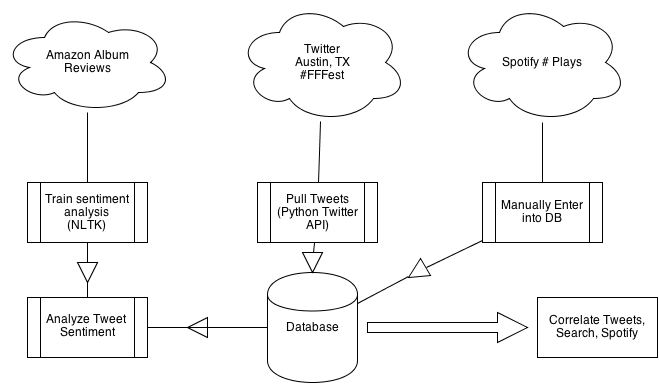
\includegraphics[scale=.5]{Flowchart.png}
\caption{Project Flowchart}
\end{center}
\end{figure}

\subsection{Twitter Streaming}
Twitter has rapidly become one of the top social networks (coincidently, Twitter first took off after debuting at SXSW, another Austin, TX event). Twitter's tagging system, brevity, and real-time nature has made it a favorite among data-miners, as it can be rapidly indexed and analyzed. \*

To capture, or mine, Twitter data, a Python script was generated that would a) connect to the Twitter firehouse, b) collect all tweets containing a specified word (funfunfunfest) in a designated geographic location (Austin, TX), and c) store the data into a database for later use. As mentioned before, the filter parameters can be adjusted to analyze any topic or location. \*

\subsection{Data basing}
It was quickly realized that the shear volume of tweets coming in would be too large to store in an array on the local hard disk drive. Moreover, a simple array would make it computationally difficult and time consuming to index and store. Enter \emph{Redis}, a No-SQl database-- also referred to as a "data structure server"-- that is stored in-memory. Redis was chosen as it is extremely well-suited for rapidly changing data, as well as being relatively lightweight. The data is stored and organized based on the artist, the timestamp, the text, and sentiment. Python streams data in and out of the database. All entries will have the following structure: 

\begin{equation}
(ID, Date, Tweet, Sentiment)
\end{equation}

\subsection{Natural Language Processing} 
While the Twitter data has been collected, a parallel process is occurring: analyzing the language used in the tweet for sentiment. By analyzing if the tweets are mentioning the artist in a positive or negative light, we can further explore the effect of live shows. Specifically, this can be used to evaluate the old adage "there is no such thing as bad press". Natural language processing is performed using an prebuilt algorithm for Python called the Natural Language Toolkit (NLTK), which uses a naive Bayesian classifier to establish sentiment. The process is as follows: first a training set is fed into the classifier, where it will "learn" which words and phrases are used in positive and negative lights. For this project, "good" and "bad" album reviews were pulled from iTunes; the reviews have both text and a star-rating which is used as a metric for good and bad albums. The trained algorithm is then fed tweets from the database, where it analyzes the sentiment and returns its result to the database. Sentiment values are real numbers bounded by [-1, 1], where negative one is strongly negative, positive one strongly positive, and zero neutral. 

\section{Results}
Over the weekend, two hashtags were followed: "funfunfunfest" and "fff8". These tweets were parsed to see if they mentioned any of the ten artists chosen. Artists of interest were those who were on stage right before a big name act who also had a relatively low volume of Spotify plays. The rational behind these criteria is that playing before a big act would theoretically expose the band to fans who were there to get in position for the following act. The low number of Spotify plays was a crucial parameter as spikes in plays could more readily be attributed to the festival. \*

A total of 740 tweets were collected, resulting in 67 mentions of the selected artists. However, most of the tweets contained only links to pictures and hashtags, not substantive commentary. This made natural language processing impossible, as there were little to no words for the algorithm to parse. Additionally, a precompiled music language corpus-- a collection of sentences used to train the sentiment algorithm-- was not available, so an attempt was made to hand-compile one-- a task that proved immensely time-consuming and difficult. Because of these setbacks, natural language processing was not used as originally intended to test the hypothesis. \*

\subsection{Analysis}
After analyzing three days of Twitter feeds, there is little to no correlation between the number of mentions an artist receives and their Spotify plays, as seen in {\bf Figure 2}.

\begin{figure}[!ht]
\begin{center}
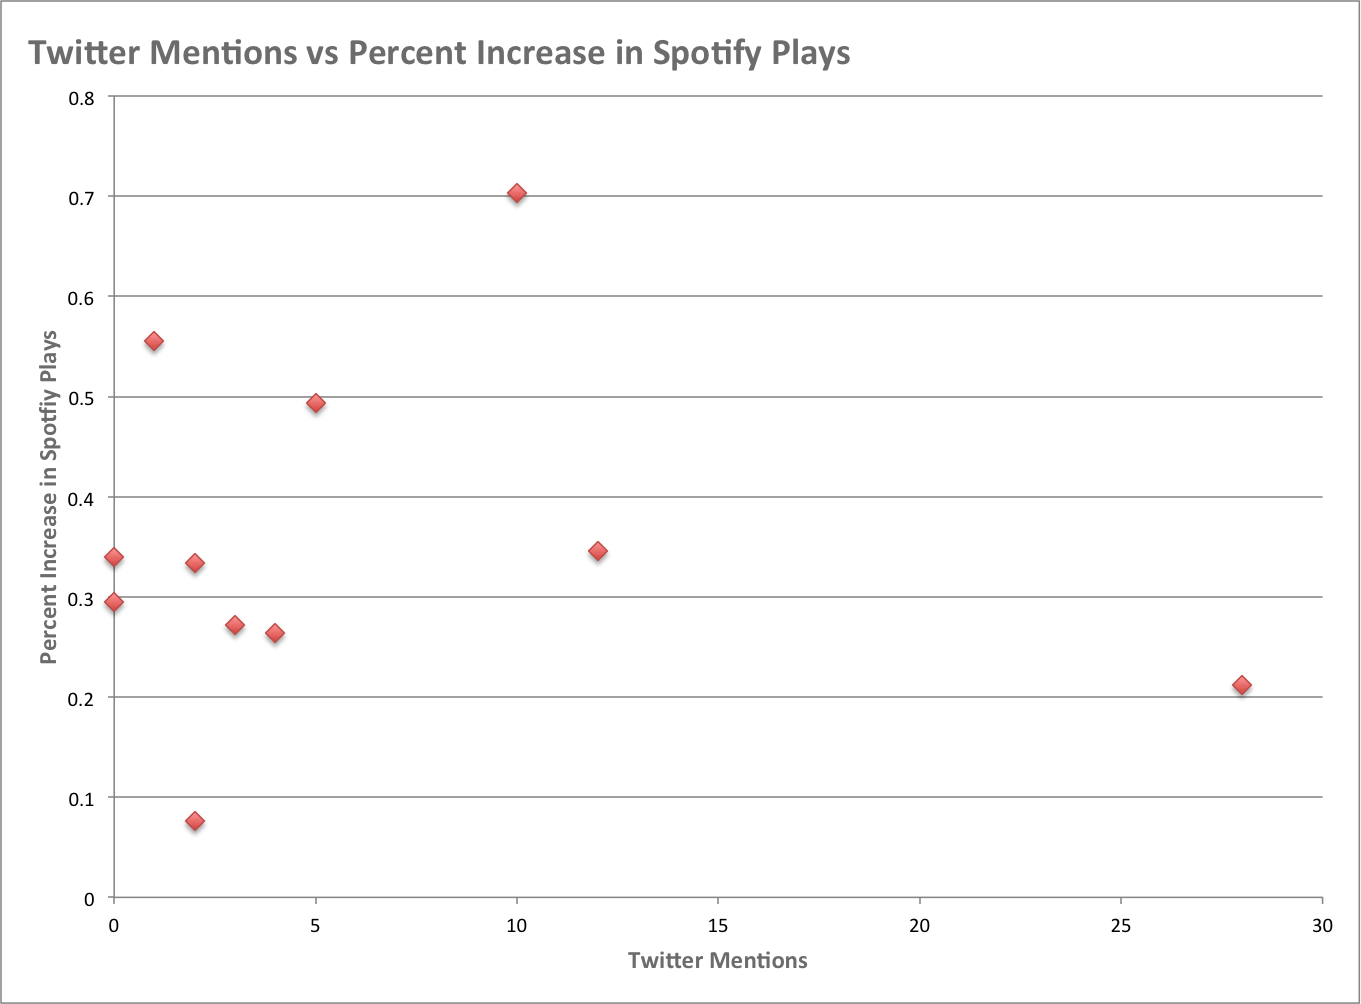
\includegraphics[scale=.6]{tweetsspotify.png}
\end{center}
\end{figure}

One possible explanation for this phenomenon (or lack-there-of) can be that attendees were excited to see bands they already knew, and while their excitement caused the fans to tweet, they did not choose to re-listen to an old favorite. {\emph{Television}} is a good example of this-- they have been together as a band for a while and while they haven't toured in years, still maintain a loyal following. Coincidently, they had the most visible rise in the Twitter-sphere. \*

There was no correlation in the volume of Google searches and the festival either ({\bf Figure 3})

\begin{figure}[!ht]
\begin{center}
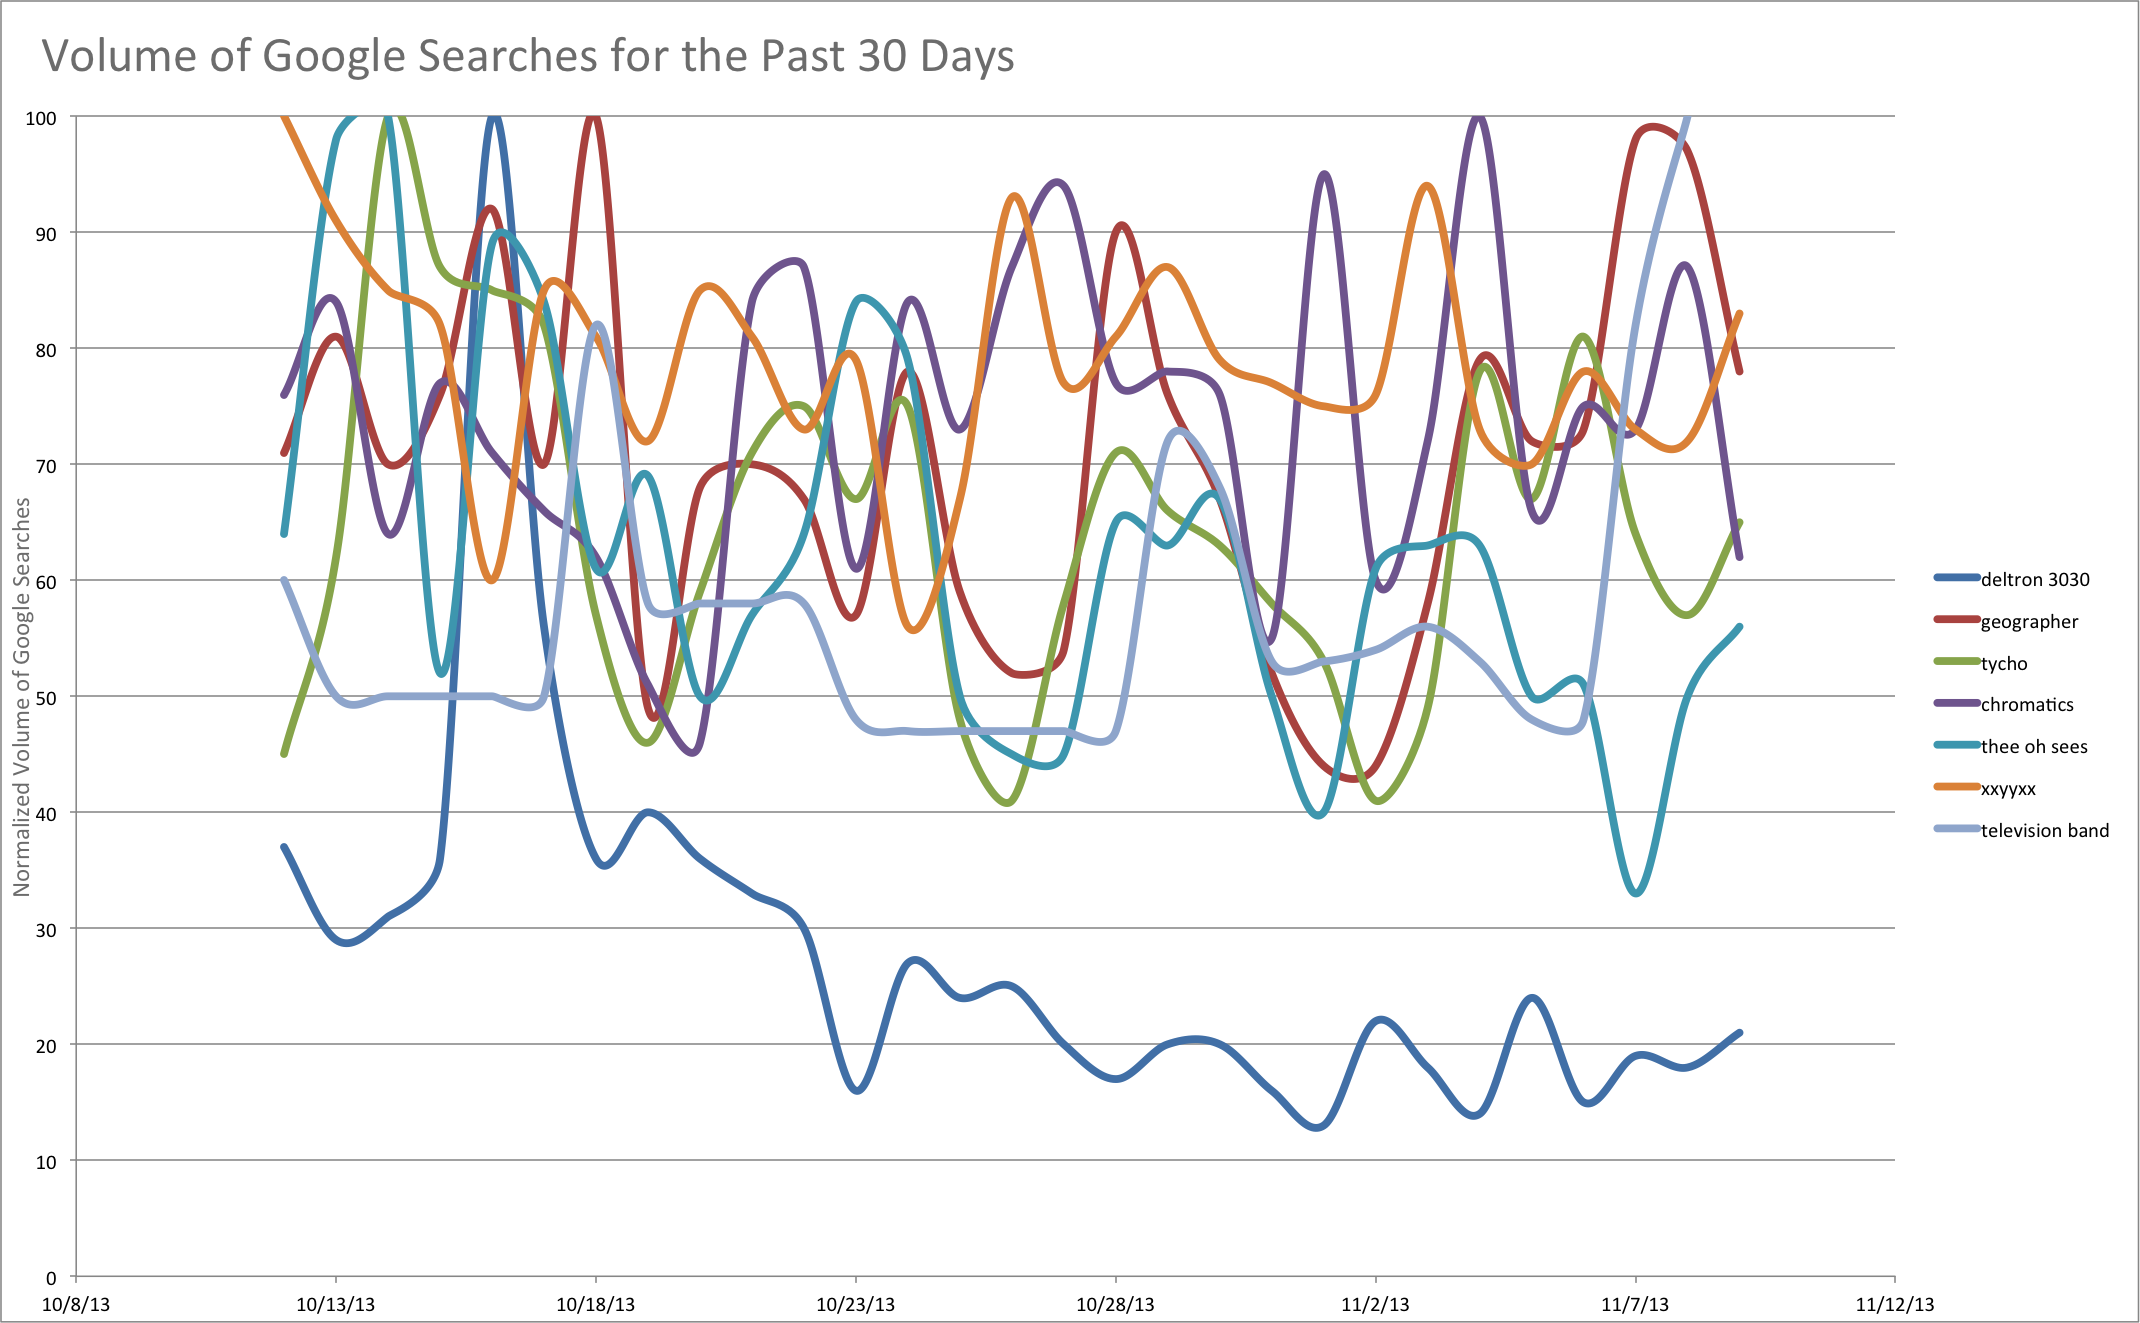
\includegraphics[scale=.5]{GoogleSearch.png}
\end{center}
\end{figure}

According to the stated hypothesis, the maximum number of searches should have occurred in the days around the festival, which was only the case for \emph{Geographer}. 

\subsection{Moving Forward}
Due to the nature of music festivals, and tweeting, Twitter-mining for artist sentiment is poorly posed, as tweets are predominantly pictures and not text. This prohibits one of the main goals of this study, sentiment analysis, from being done. Also, a large-scale corpus for music reviews would need to be complied to make natural language processing effective. However, I believe that this style of data mining could be more effective at predicting subjects that are more polarizing and contextual, such as elections. \*

Another problem in this study was the timeframes used. I think that had the artist's been tracked for a longer period before and after the event, a more revealing baseline could have been established. Instead of only measuring the number of online plays the day before, had they been tracked the two weeks before, a week before, the day before, the day of, and the week after, it could be deduced if there was a noticeable spike from baseline, as well as how many of those new listeners kept listening. \*

However, the mechanisms for parsing and storing the data worked seamlessly, and I now have a prebuilt module for capturing, storing, and filtering online data. These are tools I am confident will be handy moving forward in this class. 

\section{Appendices}

\* http://www.bizjournals.com/austin/print-edition/2012/10/05/fun-fest-happy-to-be-growing.html?page=all \*

http://nltk.org/ \*

google.com/trends


\end{document}

